\documentclass{article}
\usepackage[T1]{fontenc}
\usepackage{lmodern}
\usepackage{graphicx}
\usepackage{amsmath,amssymb}
\usepackage[a4paper,margin=2cm]{geometry}
\usepackage[absolute,overlay]{textpos}
\setlength{\TPHorizModule}{1mm}
\setlength{\TPVertModule}{1mm}
\usepackage[indonesian]{babel}
\usepackage{hyperref}
\setlength{\emergencystretch}{2em}
% unit: Halaman 39

\begin{document}

% === Halaman 39 (llm) ===

\vspace{276.21mm}

(Sumber: https://en.wikipedia.org/wiki/Stream_cipher)

% deskripsi: Tabel perbandingan berbagai stream cipher yang mencakup kolom nama cipher, tahun rilis, panjang kunci, panjang nonce/IV, panjang state, periode, serangan/kelemahan, dan kompleksitas serangan.
% bbox normalisasi: [0.0000, 0.0000, 0.8350, 0.9300]
\begin{textblock*}{175.35mm}(0.00mm,0.00mm)
\noindent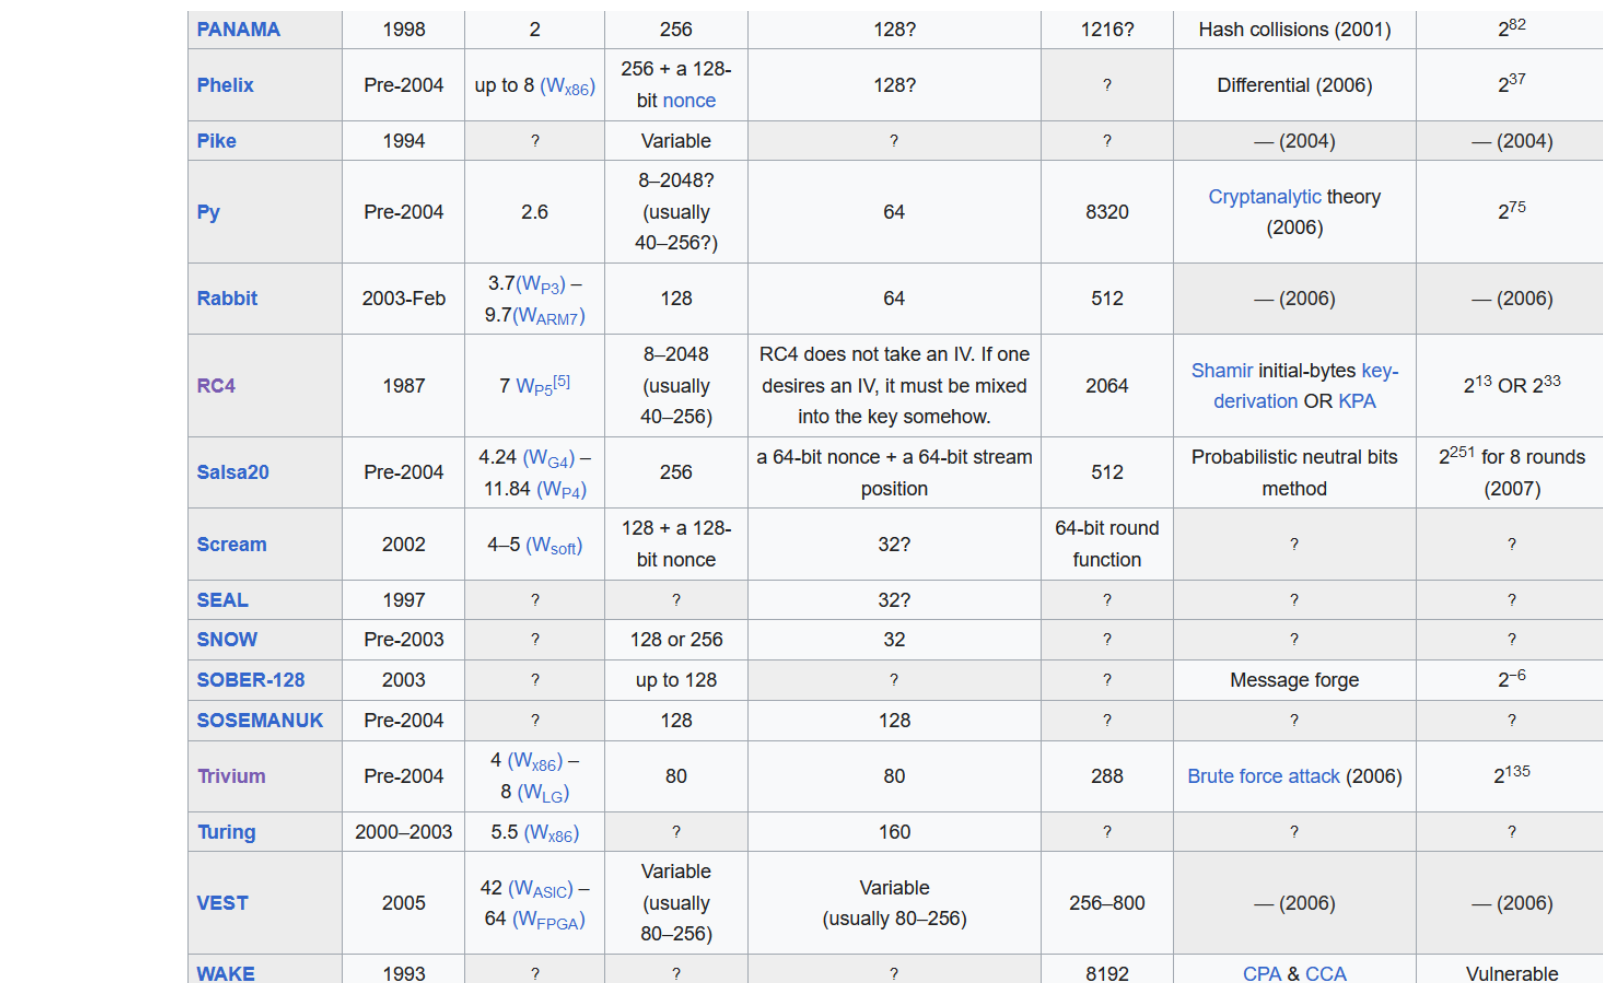
\includegraphics[width=175.35mm,height=276.21mm]{../../images/llm/page_039_img_01.png}%
\end{textblock*}

\end{document}
